\documentclass{article}
\usepackage{graphicx}
\usepackage{color}
\usepackage{comment}
\usepackage{amssymb}
\usepackage{amsthm}

\newtheorem{definition}{Definition}

%%%%%%%%%%%%%%%%%%%%%%%%%%%%%%%%%%%%%%%%%%%%%%%%%%%%%%%%%%%%%%%%%%%%%

% Algorithms and pseudo code
\usepackage{verbatim}
\usepackage{algorithm}
\usepackage{algorithmicx}
\usepackage{algpseudocode}

% Graphics and display
\usepackage{float}
\usepackage{graphicx}
\usepackage{subfig}
\usepackage{enumerate}
\usepackage{url}
\usepackage{multirow}

% Math symbols and environments
\usepackage{amsmath}
\usepackage{amssymb}
\usepackage{stmaryrd} % \varcurlyvee


\usepackage{calc}%#%

% TikZ

\usepackage{tikz}
\usetikzlibrary{shapes,arrows}
\usetikzlibrary{positioning}

\definecolor{myyellow}{RGB}{255,255,150}
\definecolor{mylavender}{RGB}{125,249,255}
\definecolor{mygreen}{RGB}{144,238,14}
\definecolor{myred}{RGB}{255,0,0}

\newcommand\mytext[3][\scriptsize]{#2\\#1 #3}
\newcommand\mynode[4][]{%
  \node[mynode,#1,text width=\the\dimexpr#2cm] (#3) {\mytext{#3}{#4}}; 
}
\newcommand\mynot[4][]{%
  \node[mynot,#1,text width=\the\dimexpr#2cm] (#3) {\mytext{#3}{#4}}; 
}

\setcounter{secnumdepth}{4}

%%%%%%%%%%%%%%%%
%%%% Macros %%%%
%%%%%%%%%%%%%%%%

%%% Math
\newcommand{\nat}{\mathbb{N}}   % Natural numbers
\newcommand{\rat}{\mathbb{Q}}   % Rational numbers
\newcommand{\real}{\mathbb{R}}  % Real numbers
\newcommand{\runit}{[0, 1]}    % The real unit interval


% = with "hip." on the top, useful for indicating where a hypothesis comes in
\newcommand{\heq}{\stackrel{\text{\fontsize{3pt}{3pt}\selectfont hip.}}{=}}
% = because of the de Morgan laws.
\newcommand{\dmeq}{\stackrel{\text{\tiny{dM}}}{=}}


%%% Sets
\newcommand{\args}{\mathcal{A}} % Set of all arguments
\newcommand{\att}{\mathcal{R}}  % Set of all attacks
\newcommand{\valueset}{L}

%%% Votes on arguments
\newcommand{\varg}{V_{\args}}   % Function giving votes on arguments
\newcommand{\vargpro}[1]{\varg^+\left(#1\right)} % Pro votes on arguments
\newcommand{\vargcon}[1]{\varg^-\left(#1\right)} % Con votes on arguments

%%% Votes on attacks
\newcommand{\vatt}{V_{\att}}   % Function giving votes on attacks
\newcommand{\vattpro}[1]{\vatt^+\left(#1\right)} % Pro votes on attacks
\newcommand{\vattcon}[1]{\vatt^-\left(#1\right)} % Con votes on attacks

%%% Attack relations
% Attackers of a given argument
\newcommand{\attackers}[1]{\att^\text{-}\left(#1\right)} 
% Attackers of a given argument for the alternative framework F'
\newcommand{\altattackers}[1]{\att^{\prime\text{-}}\left(#1\right)}
% Ancestors of given argument according to the attack relation
\newcommand{\ancestors}[1]{\att^*\left(#1\right)} 

%%% Frameworks
\newcommand{\safid}{F}               % A single SAF, given by identifier
\newcommand{\safset}{\mathcal{F}}    % Set of all SAFs

\newcommand{\saf}{\safid = \safbody} % Framework id and respective tuple
\newcommand{\safbody}{\langle \args, \att, \varg, \vatt \rangle} % SAF tuple
% Alternative framework, same as \safbody but with ' everywhere ;)
\newcommand{\altsafbody}{\langle \args', \att', \varg', \vatt' \rangle} 

%%% Semantics
\newcommand{\semid}{\mathcal{S}}        % Semantic framework identifier
% Semantic framework tuple
\newcommand{\sembody}{\left\langle \valueset,\SAFand_1, \SAFand_2,\SAFor,\lnot,\tau \right\rangle}
\newcommand{\semdef}{\semid = \sembody}     % Semantic framework id and tuple
\newcommand{\semprod}[1]{\semid^\cdot_{#1}} % Product semantic framework
\newcommand{\semsub}{\semid^\text{-}}       % Subtraction semantic framework
\newcommand{\semmax}{\semid^\text{max}}     % Max semantic framework

\newcommand{\SAFand}{\curlywedge}     % Logical and for SAF equations 
\newcommand{\SAFor}{\curlyvee}        % Logical or for SAF equations
\DeclareMathOperator*{\SAFOr}{\bigcurlyvee} % Big or notation, works as \sum
                             %\varcurlyvee also works, but is smaller
\DeclareMathOperator*{\SAFAnd}{\bigcurlywedge} % Big and notation, works as \sum

\newcommand{\modelset}{\mathcal{M}}   % Set of all models


%#% old commands
\newcommand{\afit}{\textit{AF}}
\newcommand{\af}{\afit = \langle \args, \att \rangle}
\newcommand{\vote}{V}
\newcommand{\sem}{\mathcal{S}}

\newcommand{\ssv}{\mathcal{V}}
\newcommand{\tv}{\mathcal{T}}
\newcommand{\pv}{\mathcal{P}}
\newcommand{\xv}{\mathcal{X}}
\newcommand{\ev}{\mathcal{E}}

\newcommand{\safit}{F}

\newcommand{\tupd}{\curlywedge}
\newcommand{\tatt}{\curlyvee}
\newcommand{\Tatt}{\varcurlyvee}

\newcommand{\argarray}{\{x_1, ..., x_n\}}

\newcommand{\voteset}{\mathcal{V}}
\newcommand{\vpro}{\vote^+}
\newcommand{\vcon}{\vote^-}

%%% Mappings
\newcommand{\mapping}{\Phi}

%%%%%%%%%%%%%%%%%%%%%%%%%%%%%%%%%%%%%%%%%%%%%%%%%%%%%%%%%%%%%%%%%%%%%
%%%%%%%%%%%%%%%%%%%%%%%%%%%%%%%%%%%%%%%%%%%%%%%%%%%%%%%%%%%%%%%%%%%%%

\begin{document}

\title{Pointers for collaboration}

\maketitle

This document tries to draw a rough roadmap in order to extend the framework defined in \cite{leite2011social}.
%contains some pointers in order to extend the framework defined in \cite{leite2011social}
\\
\section{The concept of support} 

%%{\color{red} }
%the intuitive idea
%%Embedding the concept of support relations in our system carries utmost importance.


%the objective:
In the current state, of our system there is no concept that could be directly mapped to the notion of support relations as in the works like \cite{DBLP:journals/ijis/AmgoudCLL08}. The only ways of realising indirect support in Social Abstract Argumentation would be casting negative votes to the attackers of the supported argument, or in a similar sense to cast positive votes in favour of the attackers of the attackers or by introducing some new arguments attacking to the original attackers. Here the discussion is on if the system could benefit by having a more comprehensive mechanism with respect to the notion of support. We will elaborate on a handful of potential approaches under this topic.

%methodologies:
%meth1 - support branch
\subsection{Support branch}
Incorporating the notion of support is not a trivial matter and therefore one should carefully consider whether the realized method shows ingenuity and brings some clear advantage. 
%For instance, in \cite{gradinarg} authors try to capture the notion of support via \textit{paths}. 
For instance, the work in \cite{gradinarg} is based on the idea that indirect defenders are in fact supporters, and thus help strengthen an argument instead of minimising the damage done by an attacker. In this situation, it may happen that an argument attacked by more arguments may be stronger than one without certain attacks. The reason is that certain attackers may actually belong to a support path. In their work, a path from an argument to another is said to be an attack branch if its length is odd and a support branch if it is even. 

By emphasising the role of support branches in their global approach, it happens that argument $a$ is stronger in Figure \ref{subfig:wsup} than in Figure \ref{subfig:wosup}. This is because $a$ has one support and one attack branch in \ref{subfig:wsup}, and one attack branch and no support branch in \ref{subfig:wosup}. We do not share the same sentiment with this school of though, and actually argue the opposite. If one adds an attacker to argument $a$, then $a$ should not become stronger under any circumstances. And if this attacker is in turn attacked, it should only mean that the original attack was in fact a weak one, but not one that can be turned into support. Imagine, for example, that c is a fallacious argument, which is promptly attacked by d (an argument that simply points out that c is fallacious). Why should the value of "a" increase over the situation where it was simply not attacked by "c"?

So all in all, it shouldn't matter whether there is a support branch: another attacker means further evidence that the attacked argument is not true. From this point of view, the best case scenario for $a$ would be for the new attacker to be defeated and $a$ maintaining its degree of truth. This illustrates two very different intuitions which do not seem trivially reducible to one another, if at all.

\begin{figure}[h!]
  \centering
  \subfloat[An argument with one attacker, without  support]{
    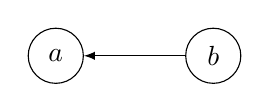
\begin{tikzpicture}[>=latex, auto]
  
    \tikzstyle{argument}=[draw, shape=circle, minimum size=7mm];
  
    \node [argument](a) at (0, 0){$a$};
    \node [argument](b) at (2, 0){$b$};
  
    \draw [->] (b) to (a);

    \end{tikzpicture}
    \label{subfig:wosup}
  } \hspace{1cm}
  \subfloat[Same argument with one support branch]{
    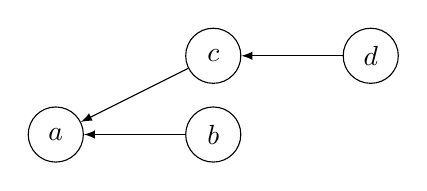
\begin{tikzpicture}[>=latex, auto]
  
    \tikzstyle{argument}=[draw, shape=circle, minimum size=7mm];
  
    \node [argument](a) at (0, 0){$a$};
    \node [argument](b) at (2, 0){$b$};
    \node [argument](c) at (2, 1){$c$};
    \node [argument](d) at (4, 1){$d$};

    \draw [->] (b) to (a);
    \draw [->] (c) to (a);
    \draw [->] (d) to (c);

    \end{tikzpicture}
    \label{subfig:wsup}
  }
  
  \caption{Addition of  a support branch according to \cite{gradinarg}}
  \label{fig:oops}
\end{figure}

%meth2 - support relation
\subsection{Support relation}
There are also works(e.g. \cite{4}) which consider the attack and support relations as being independent and very much dual. So crudely a support relation is also a mapping between two arguments, but where the starting point enhances the strength of the ending point, rather than diminishing it. We continue our discussion by debating the added value of this concept. 

 Suppose a simple example where $a$ supports $b$. The idea here is that if $a$ supports $b$, or in other words if $a$ is evidence for $b$, then to defeat $b$ one must first defeat $a$. Until there is no support or evidence for a given proposition, that proposition must be true. A set of supporting arguments can be seen as a conjunction, disjunction or mix of facts (the premises) that lead us to believe the conclusion (the argument which they support). The most obvious and direct solution for removing the support relation is to replace all these arguments with a new, structured argument. Its premises can be the supporting arguments (most logics trivially accommodate conjunctions, disjunctions or a mix as premises). Then, any argument that previously attacked a supporting argument can be considered an undercutting attack while any argument previously attacking the conclusion can be seen as a rebutting attack. Obviously, this is a simplified procedure, but nonetheless seems feasible. Once again, it is possible to remove the support relation from a framework, without altering its intended semantics. This previous argument seems to indicate that the two relations are not symmetric in nature. 

We must note with respect to capturing the support notion in our system, support relations might indeed be the way to go. However currently we are still motivated to look for alternative methods.

%meth3 - pro arguments
\subsection{Pro-arguments}
In the light of prior discussion, a new methodology to achieve this objective is an extension of the current framework with a notion of \emph{Pro-arguments}. In the sense that, instead of defining the counterpart of binary attack relations, the so-called support relations, we consider the new concept of pro-arguments,  which would be of a somewhat different nature, more in line with structural parts of the arguments they defend rather than stand alone arguments. Therefore the correlation will not be realised via a binary relation, but pro-arguments will simply be attached to their corresponding arguments\footnote{Let us call these arguments as base arguments.} as internal structures. 

Therefore in this first take of the method, the social voting still will only take part on the arguments themselves, thus these structures should be interpreted as additional reasons to make users vote on that particular argument. It appears that pro-arguments could easily be added in the mix without making the GUI more complex. Perhaps a good approach would be embedding the pro-arguments into their associated argument. In the sense that one would only reveal them by clicking on the base argument, graphically in a similar way \textit{debategraph.org} displays the sub-relations of an argument. 

In all truthfulness, this approach is an enhancement more on the GUI side, rather than the theory. The gist of the idea is that pro-arguments potentially constitute new motivations for users to vote on their associated arguments.  If the users do not agree with a particular pro-argument, they're simply assumed to ignore it. So they're just a tool for getting more positive votes(and similarly less negative votes) for the base argument, but mathematically they don't have a direct effect on the social strength of the base argument. Not surprisingly, a viable question would be: How about letting users vote on pro-arguments as well?

When we treat pro-arguments as first-class citizens, or in other words when social voting also applies to them, challenges may occur. Suppose the following simple example: There is an argument $a$ in an instance of our framework which has received 100 positive votes and 0 negative votes. Then three pro-arguments are introduced to the framework where they are associated to argument $a$. All of these pro-arguments get 0 positive votes and 20 negative votes. Now all of a sudden as a result of these socially unwelcome pro-argument, should the social strength of $a$ diminish? In sum, the way that the system handles the computation of the social strengths in such a setting, possess a tricky yet highly interesting problem.

One final idea related to this approach is: defining a vector for each argument in the system, and representing the aggregated strength of the Pro-arguments as one dimension of this vector. Here we omit to go into details regarding this method as it will be discussed in Section \ref{mulDim}.


%meth4 - no negative votes
\subsection{Without negative votes}
Lastly, a naive alternative could be constructing a system without negative votes. Thus whenever a user is in favour of an argument, s/he will be casting a vote on the argument. So we maintain the notion of support realised as  a direct concept through votes. On the other hand if the user detests an argument, then s/he should find a counter argument to attack it, specify it by utilising the means of the system and then vote on the argument and the attack as well. This simply equates to only updating the mappings regarding the voting mechanisms of our framework.

Since this approach is based on the idea of expelling the negative votes from the system, the mappings only keep the positive votes for arguments and attacks. Of course now there is a need for modifying the vote aggregation functions as well since the set of parameters have changed. One can experiment with different choices of functions, perhaps the most obvious one being: for an argument $a$, the social support value $\tau(a) = v(a) / v_{max}$ (where  $v_{max}$ stands for the maximum number of votes for an argument in the system). Thus only the argument(s) with the most number of votes in the framework would enjoy perfect social support. Other possible alternatives could include the total number of voters (if the system has logged users), or the total number of voters for that particular debate (connected graph), or some local measure (total number of voters in the subgraph composed of the arguments which are no further away than some distance and so on.


In the case of this methodology, it does not seem like serious technical difficulties would arise. This prospect is indeed plausible, since the approach is a simplistic state of our existing framework. As the social voting  is still solely on arguments, the method does not force us to make any changes regarding the fundamental procedures of our system.
The most obvious potential criticism regarding this method  may point to the fact of the system lacking negative votes, as this had also been a major source of discontent for a vast amount of Facebook users \cite{FBdislike}. 


\section{Representing multi-dimensional dataset} 
%the intuitive idea
Displaying multivariate data of our framework via a multi-dimensional graph presents a challenge with respect to the ease of comprehension for the human users.

%methodologies:
An unorthodox yet interesting method that we may utilize, instead of using mere size and color changes of arguments, is the \textit{Chernoff faces}. They were first proposed by by Herman Chernoff \cite{Chernoff73} in 1973, as a way to represent multivariate data in a manner that is easily discernible by the human viewer.  The whole reasoning behind the use of Chernoff faces relies on the claim that humans are adept at face recognition and are able to notice reasonably acute changes in facial characteristics. The faces consist of two-dimensional line drawings that contain a variety of facial features. Moreover these facial features can be mapped to different dimensions in a multidimensional data set. The individual parts, such as eyes, ears, mouth and nose represent values of the variables by their shape, size, placement and orientation. In a similar sense, our approach would be mapping concepts from our framework such as  \textit{the social support of the argument, the social strength of the argument, the number of total votes that were casted on the argument and also the number of attacks that argument was being subjected to}, to distinct facial features. One notion that requires attention is that Chernoff faces handle each variable differently and because the features of the faces vary in perceived importance, the way in which variables are mapped to the features should be carefully chosen (e.g. eye size and eyebrow-slant was found to carry considerable weight compared to rest \cite{Morris00}).

%difficulties
In literature, there are mixed sentiments towards the validity of Chernoff faces. For instance in \cite{Morris00} authors claim that their experiments clearly depict that the use of Chernoff faces for information visualization does not take advantage of human pre-attentive visual processing, that Chernoff face feature perception is solely a serial process and not pre-attentive. Since the existing experiments do not seem to be decisively conclusive for neither schools of thought, perhaps the real value of Chernoff faces' use if our system can be best evaluated by carrying out our own tests.


\section{Distinct voting schemes}
%the intuitive idea
Our system does not have any assumptions on the intrinsic meaning of a \textit{negative vote}, however distinguishing and handling the notions accordingly might prove to be fruitful.

%methodologies & GUI difficulties:
%% 1p, 2n
Automatically recognizing different schemes of negative votes is a challenging problem. However if the classification can be made, it might be more plausible to use different operators in our system regarding their utilization. So in summary, the focus is on the question of whether a negative vote means the argument is badly spelled out, or simply the user does not like the conclusion of  the argument. One methodology here can be rather than relying on automated mechanisms for capturing types, distinctly specifying the two types of negative votes and their related operators, and giving sufficient means to the users so that they can manually point out the intended meaning in our system. 

This technique consists a unique support vote. The underlying assumption is when a positive vote is casted on a particular argument, the intuition is that the user agrees with the conclusion of the argument. Hence with respect to this method, we could extract all the information from the users by just letting them having three buttons to push in the GUI: One for positive, one for negative on the structure and one for negative on the claim. And of course they're allowed to push both of the latter buttons in case they're dissatisfied with both the structure and the claim.

%% 2p, 2n
An alternative approach may try to answer the following question: How should a user vote if the argument is well spelled out and the user does not agree with the conclusion? Even that our framework deals with abstract arguments, perhaps many textual arguments will consist of some premises, some support and a conclusion. In the system, some arguments may prove to be fallacies, such as: "Hitler was a vegetarian, thus being a vegetarian is a healthy life choice".  Most probably, many users would agree with the conclusion of the argument. At the same time many could complain on the structure because of the flawed logical entailment of  the premise.

In the light of this idea, voting schemes boil down to two dimensions. In GUI, the neccesasary information can be simply gathered from the users with the following \textit{yes/no} questions:
\begin {itemize}
\item Is the argument well structured?
\item Do you support the claim?
\end{itemize}


%Challanges in formal framework
Extending our framework with either of these methodologies invoke some challenges concerning the formal framework. The main purpose of our framework is evaluating a strength for each argument via utilizing the social voting as input. Consequently mashing up the information gathered from the two distinct voting schemes on the conclusion and the structure of the arguments, requires some elegant mathematical solution.



Another challenge that transpires by the discussion of the different interpretations of votes is the concept of inconsistency with respect to the votes casted by a certain user. Since the system constantly evolves, two arguments that a specific user was in favor of can all of a sudden be attacking to each other as a consequence of the introduction of some attack relation by another user. On the other hand, if the interpretation of the votes is taken as an argument being well-structured or not, then it's perfectly plausible to cast "positive votes" on two mutually attacking arguments.

%difficulties(not so much)
Lastly, we may conclude that tests carried out via interacting with human users would be critical to gain some insight on the dominant preference regarding the  schemes. 



\section{Multi-dimensional vote definition}
\label{mulDim}
%the intuitive idea
In addition to the ratio of positive and negative votes, the total number of votes an argument has must be a significant parameter, when the system comes up with the final evaluation.

 In our existing system, the model of an argument is computed by roughly crunching  the number of positive and negative votes the argument has received into a single value in  $[0,1] \in \mathbb{R}$. There has been some early efforts in order to remedy this notion, specifically for incorporating the effect of number of total votes into our vote aggregation function. For instance with the following definition:

%\newpage
\begin{definition}
[Vote Aggregation]A vote aggregation function is any function
$\tau:
\mathbb{N} \times \mathbb{N} \times \mathbb{N}
\rightarrow\lbrack0,1]$ such that $v_{max}\geq0$
\[
\tau\left(  v^{+},v^{-}, v_{max}\right)  =\left\{
\begin{array}
[c]{lll}
0 &  & v_{max}=0\\
\frac{v^{+}}{v^{+}+v^{-}+\frac{1}{v_{max}}} &  & \text{otherwise}
\end{array}
\right.
\]

where $v_{max}$ stands for the maximum number of votes for an argument in the system.
\end{definition}

already is sufficient to prove some desirable properties(wrt. specific context) such as \textit{"If the value of the ratio of positive votes to the total amount of votes is higher for an argument $a$ than an argument $b$; $a$'s social support value exceeds the social support of $b$"} and \textit{"When the ratios are equal, the function should return a higher social support value for the one with the higher number of total votes"}. Those being said, there might be a need for a more complex methodology in order to incorporate the total number of votes to our framework.


With the inspiration of \cite{baroniTAB13}, in our system votes might be defined as vectors in bi-dimensional space. So simply put, the idea is defining the social support of an argument in a way that it's not anymore solely a function of the relative magnitude of positive and negative votes the arguments have received. In other words, instead of collapsing positive and negative votes into a single value and utilising it,  we specify the votes as vectors and operate on them via some vector operators. A possible choice of vector components is letting number of positive votes be one component, and the number of negative votes the other. 

In the original work \cite{leite2011social},  an argument with 4 positive and 3 negative votes would roughly enjoy the same social support value of an argument with 60 positive and 45 negative votes. By the aforementioned vector approach and component pair selection, now the two social support values would approximately differ by a factor of 15 as a result of the relative magnitudes of the two vectors. In contrast to the original definition, the effect of the total number of votes an argument has received is significantly reflected in its strength values.

Interestingly, an extension with this notion does not require a change in the overall framework as the labeling sets(where the arguments values come from) and the operators are defined as purely generic. In other words, there are no restrictions in the framework that would prevent us from taking the values as vectors. So in this scenario we may choose the argument values as vectors, select the algebraic operators as some set of vector operators, and at the end the result(i.e. the model of the framework) would be a set of vectors. Consequently we enjoy a new level of expressiveness since we have the flexibility of representing the vectors whatever way proves to be interesting.

Moreover there might be also other alternatives for the components of the vectors. For example we may choose one component to reflect the relative measure of the positive and negative votes of a specific argument(which resembles the idea behind the original social support definition). This can be achieved taking the ratio of positive votes over negative votes, the ratio of positive votes over total number of votes, the absolute difference of the positive and negative votes of the argument, and so on. On the other hand, we may select the other component to stand for the size of the total number of votes for a specific argument. Conceivably, the sum of positive and negative votes can be associated for the mentioned value.

A concern regarding such an approach is that: Even that the components express two different notions, formally the functions that give birth to these values contain the same inputs. Namely the positive and negative votes of the associated argument. This can impose a restriction on the directions that the argument vector can take in 2D Cartesian-space, since the two values are mathematically bounded by each other rather being independent components.

Lastly we should note that a bi-dimensional approach is not the only way to go. It might make sense to keep an eye out on the related topics for some inspiration regarding new dimensions, and extending our multi-dimensional method by utilising them. For instance in Section 1, we discussed a few techniques for incorporating the notion of pro-arguments. For all of them, we were able to list some potential caveat. Perhaps pro-arguments can be captured better as the third component of our first methodology under this section. Thereupon an argument is represented as a 3D vector where the components are the positive votes, the negative votes and the support of the pro-arguments that particular argument gathered. 
 
\section{Strategic Voting}
%the intuitive idea
In order to demonstrate how prone our system is against manipulation, studying strategic voting is truly important.

Our system is going to be utilized by human users. Undoubtedly they are going to be acting as self-interested entities and try to capitalize on opportunities in which they man manipulate the system and get closer to their preferred outcome. Ideally we would like to be able to assure the confidence of the users in the sense that they wouldn't have to any incentive to worry about strategic reasoning and the ways they choose to vote. They could simply vote on the arguments and attacks they like and that would be the best thing they could do in terms of their desired outcome. Such a state with respect to the field of voting systems is a utopia and indeed formally proven to be impossible \cite{arrow}. Having said that, there are works in the literature which dwell with related notions to this subject. One example is the concept of \textit{price of anarchy}  \cite{koutsoupiasP99}, which provides a measure of how much a system degrades due to self-centric acts of its agents.

%methodologies:
For the purpose of finding out the behavior patterns of users in our system, we may benefit from devising different settings of the system and running simulations and live tests by utilizing those.  

For instance, we would expect some users to have a subset of arguments in their minds that they want to promote in the framework. So perhaps one parameter of our setting could be based on this notion. There are works in the fields of Social Choice Theory and Voting Theory that might help us. For example \cite{bonzonmaudet11} inspects a scenario where each agent has a specific preference on one particular argument in the system, named as \textit{the issue}. The agents try to mold the system with respect to their own preference on the issue, by utilizing the pre-defined rules. We could surely benefit from adopting their ideas, however in our setting it would probably make sense that the users have multiple issues. 

Firstly as in \cite{bonzonmaudet11}, we may choose to partition the users into different groups with respect to their shared issues and pursue the study by pointing out the actions of the parties. On the other hand we may have a more flexible setting by letting each user have their own set of preferences. Moreover preference vector might be defined for each user that either ranks arguments, constitutes a subset of arguments that the particular user would like to maximize the sum(or the result of some other aggregate function) of their values. 

In the light of this discussion, a related notion is the introduction of a budget concept on votes. Roughly the idea is allotting users a certain amount of vote to be casted on the arguments and attack relations. So in this setting, since the votes the users possess is finite, they are forced to make a set of rational selections between the available choices. Probably the motivation that would drive these decisions would be based on the preference vector mentioned above. 
We may also choose the adopt the concept of budget on some other notions as well. Perhaps we may limit the number of new arguments and attack relations that a user may specify. We may choose to increase the budgets of the users, whose introduced entities surpass a certain threshold of positive votes; hence we can also assure there is always some potential incentive for the users to come back to a debate they participated earlier. 

%difficulties
\cite{bonzonmaudet11} elegantly displays that figuring out the expected user behavior could be highly challenging, even in a setting where the whole system contains a single issue. Having multiple issues in the system, and moreover multiple arguments even in the case of a single user's preference list would surely increase the difficulty to new levels. All in all, the subject of strategic voting in social argumentation systems is surely intriguing but also a highly demanding problem. Thus construction of a handful genuine settings, that are also computationally tractable carries utmost importance.

%additional enhancement
Lastly on a different note, another idea which relates to the aforementioned topics is inspired by \cite{maudetComma}. The authors choose to work with a method that utilizes labeling users and keeping a track of their contributions on the system with respect to their expertise. Thus one may easily establish the distinct ways different user groups affect the system. Embedding of this idea is certainly worthwhile.



\bibliographystyle{plain}
\bibliography{BTCcollaboration}

\end{document}